\begin{tikzpicture}[remember picture,overlay]
\thispagestyle{empty}
  \node at (current page.center) {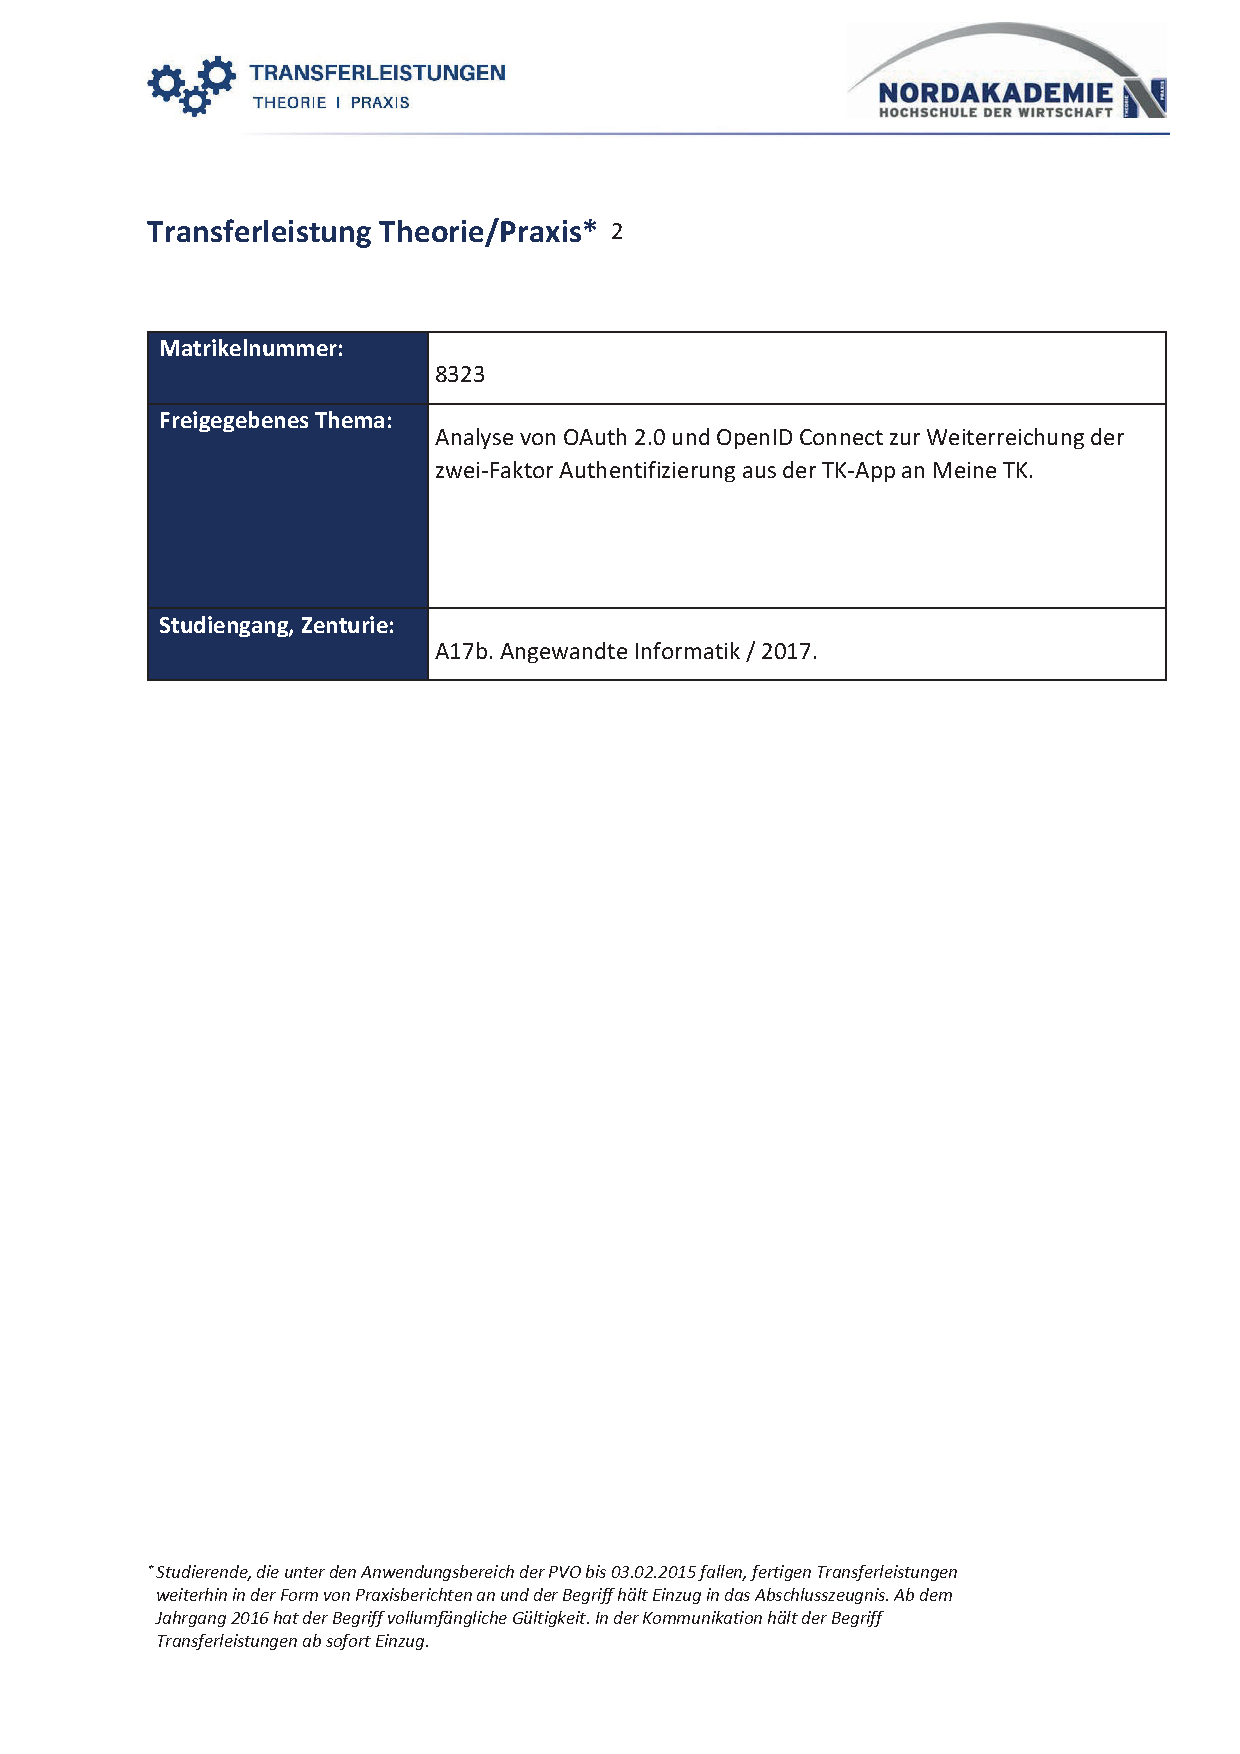
\includegraphics[page=1]{misc/deckblattTerminiert.pdf}};
\end{tikzpicture}
\newpage
% Klassische Titelseite

\thispagestyle{empty}
\begin{center}
\vspace*{-2cm}

\includegraphics[width=0.85\textwidth]{Bilder/Logo_NAK}\\
\vspace*{3cm}
{\color[RGB]{91,155,213}\hrule
    {\fontfamily{put}\selectfont \huge \onehalfspacing
    \color[RGB]{91,155,213}\thetitle
    \par}%
\hrule}
   \vfill
  %\vskip 6em
    {\normalfont\normalcolor\bfseries
	\large
	Transferleistung \\
	\large
	im Studiengang Angewandte Informatik\\
	angefertigt im Projekt-Team Innovations.OMP\\
	der Techniker Krankenkasse\\
    \par}%
\end{center}\par
%\vfill
\vspace*{2.5cm}
\noindent\begin{minipage}[b]{\textwidth}
{
  \noindent \textbf{von \theauthor, geb.~am 01.~März 1998 in Bad Oldesloe}\\

  \begin{tabbing}
  \textbf{1. Betreuer und Pr\"ufer:}  \= \textbf{Jan Koops, Tech-Lead TK-App}\\
  \textbf{2. Betreuer und Pr\"ufer:}  \= \textbf{Philip MacDonald, Full-Stack/IOS}\\
  \textbf{3. Betreuer und Pr\"ufer:}  \= \textbf{Jan Ove Weichel, Android}\\
  \end{tabbing}

  \noindent \textbf{Hamburg, den \thedate}
  }
\end{minipage}
 \newpage \thispagestyle{empty} \addtocounter{page}{-3}
\setlength{\evensidemargin}{0.6cm}			%Zum Drucken -0.6cm Rand einstellen!
\setlength{\oddsidemargin}{0.6cm}				%Zum Drucken 0.6cm Rand einstellen!
\begin{abstract}[Abstract] \thispagestyle{plain} \fussy Semiconductor-2nanowires
(NW) are one of the smallest lasing sources and thus gained a lot of attention
in order to achieve the required future miniaturization of optoelectronic
devices. Light-matter interaction in NWs and their angular emission distribution
are determined by the operating transverse laser mode which defines the
polarization of the propagating light. Since single zinc oxid NWs provide gain
material combined with a Fabry-Pérot-Cavity, coherent laser emission can be
achieved by optical pumping. The laser emission is most pronounced at the
endfacets such that both interfere similar to a Young's double-slit experiment.
The emerging pattern is analysed via Fourier optics in angular-resolved
Microphotoluminescence. In addition to this, Stokes parameters of the emitted
light can be determined spectrally resolved for individual modes, giving an
insight into the field distribution in the NW. Using external magnetic fields,
changes in laser and emission characteristics are analysed. Thus, nanowires were
transfered to a magnetizable substrate and with a Helmholtz coil allowing to
change the direction of magnetization \textit{in situ}, spin polarization was
striven for using spontaneous spin coherence caused by proximity effects.
\end{abstract} \newpage \thispagestyle{empty}
\begin{abstract}[Kurzzusammenfassung] \thispagestyle{plain}
\addtocounter{page}{-1} \fussy Halbleiternanodrähte gehören zu den kleinsten
bekannten Lasern und sind somit interessant, um in Zukunft die erforderliche
Miniaturisierung von optoelektronischen Anwendungen voranzutreiben. Die
Wechselwirkung zwischen Licht und Materie in Nanodrähten und die
Winkelverteilung der Emission werden maßgeblich durch die transversale Lasermode
determiniert und damit auch die Polarisation des Lichtes festgelegt. Da Zinkoxid
Nanodrähte ein aktives optisches Medium darstellen und gleichzeitig als
Fabry-Pérot-Kavität fungieren, kann kohärente Laseremission durch optisches
Pumpen erreicht werden. Hierbei konzentriert sich die Laseremission
hauptsächlich auf die Endfacetten, die, ähnlich dem Young'schen
Doppelspaltexperiment, interferieren. Dieses Interferenzmuster wird via
Fourieroptik in winkelaufgelöster Mikrophotolumineszenz analysiert. Hierüber
hinaus werden die Stokes-Parameter der Emission spektral aufgespalten für
einzelne Longitudinalmoden betrachtet und erlauben somit einen Einblick in die
Feldverteilungen im Nanodraht. Unter angelegten externen Magnetfeldern wurden
Veränderungen der Laser- und Emissionscharakteristika untersucht. Hierzu wurden
die Nanodrähte auf ein \mbox{magnetisierbares} Substrat aufgebracht und die
Magnetisierungsrichtung mit einer \mbox{Helmholtzspule} \textit{in situ}
verändert. Hierbei soll der ``\mbox{Proximity}-Effekt'' für eine spontane
Spinkohärenz sorgen, die zu einer Spinpolarisation führt. \end{abstract}
\setlength{\evensidemargin}{0cm}			%Zum Drucken -0.6cm Rand einstellen!
\setlength{\oddsidemargin}{0cm}				%Zum Drucken 0.6cm Rand einstellen!
\tableofcontents \newpage \thispagestyle{empty}
%\listoffigures
%\listoftables
